\chapter{Einleitung}
In der heutigen Welt werden täglich große Datenmengen erzeugt siehe dazu
Abbildung \ref{fig:data-grow}. Sei es im privaten Umfeld durch die Benutzung
von Social-Media-Plattformen wie Facebook, Twitter,~\dots{} oder in der
Wirtschaft durch Börsendaten, medizinische Bilddaten,~\dots . Im Zuge der
zunehmenden Vernetzung von Alltagsgegenständen wie Fernseher,
Kühlschrank,~\dots{}, welches man auch als IoT\footnote{Internet of the Thinks}
bezeichnet, stieg die täglich erzeugte Datenmenge noch einmal sehr stark an.

\begin{figure}
\centering
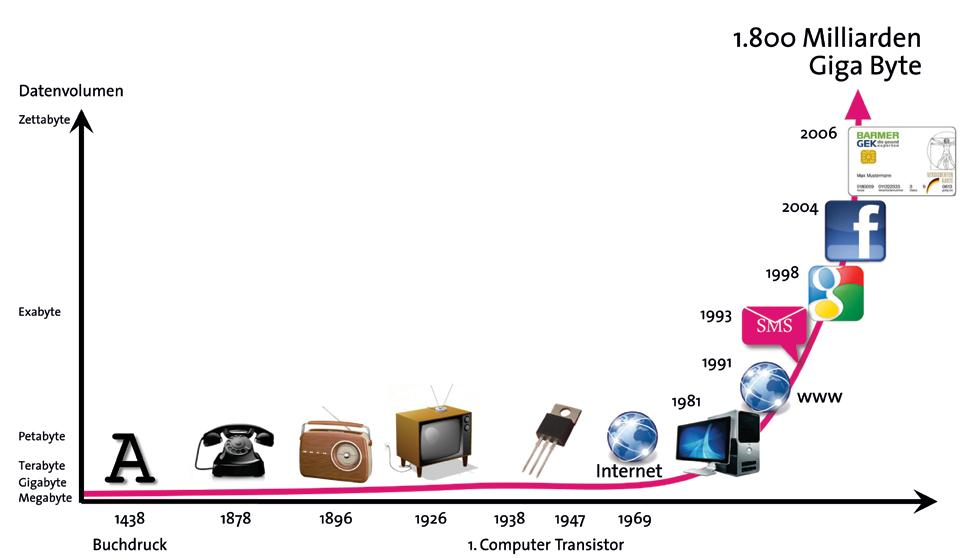
\includegraphics[scale=0.375]{images/bitkom-lf-bigdata-2012-data_grow.jpg}
\caption{Erhöhung der Datenmenge von 1400 bis 2006 \cite{Weber2012}}
\label{fig:data-grow}
\end{figure}

Diese Daten können dabei strukturiert, semi-strukturiert oder unstrukturiert
sein. Strukturierte Daten können sehr leicht von Maschinen verarbeitet werden,
da sie über eine fest vorgegebene Struktur verfügen. Im Gegensatz dazu haben
semi-strukturiete Daten eine lose Struktur, dies bedeutet, dass definiert ist,
wie einzelne Bausteine auszusehen haben, jedoch nicht wie das Dokument aus den
definierten Bausteinen entsteht. Über unstrukturierte Daten kann man lediglich
die Aussage treffen, um welchen Typ von Daten es sich handelt, also zum
Beispiel, ob es ein Bild ist.

Diese riesigen unterschiedlich strukturierten Daten müssen effizient
gespeichert und verarbeitet werden, damit ein Mehrwert entstehen kann.
Relationale Datenbanksysteme stoßen dabei schnell an ihre Grenzen. Für solche
Zwecke ist es besser, alternative Systeme einzusetzen wie NoSql-Systeme.
% TODO: Begründung

\section{Motivation}
Wie schon erwähnt, sind NoSql-Systeme bei semi- und unstrukturierten Daten besser
geeignet. Jedoch gibt es eine Vielzahl von unterschiedlichen NoSql-Systemen,
die alle für einen gewissen Einsatz entwickelt wurden. Um deshalb eine
Entscheidung treffen zu können, welches System man einsetzen möchte, muss man
die verschiedenen Systeme vergleichen. Dabei spielen nicht nur die Funktionen
der einzelnen Systeme eine Rolle, sondern auch eventuell vorhandene
Bibliotheken.

Im weiteren Verlauf dieser Arbeit werden wir die Schlüssel-Wert-Systeme als einen
Typ herausnehmen und davon mehrere Systeme und deren Integration vergleichen.

\section{Ziel der Arbeit}
Ziel der Arbeit ist es, die Schlüssel-Wert-Systeme
Redis\footnote{\url{http://www.redis.io}},
Memcached\footnote{\url{http://www.memcached.org}} und
Voldemort\footnote{\url{http://www.project-voldemort.com}} hinsichtlich ihrer
Eigenschaften zu untersuchen. Dabei soll vor allem der Fokus auf
Leistung\footnote{Performance} und verteieltes Rechnen\footnote{Clustering}
gelegt werden. Redis verfügt über ein eigenes System \enquote{redis-benchmark},
welches ausgeführt und mit den eventuell vorhanden Werkzeugen der anderen Systeme
verglichen werden soll. Dabei kann es notwendig werden, das Werkzeug für die
anderen System anzupassen.

Außerdem sollen die existierenden
Zugriffsbibliotheken\footnote{Client-Libraries} der Systeme verglichen
werden. Der Fokus soll hierbei auf der Programmiersprache Python liegen. Dazu
sollen geeignete Anwendungsfälle ausgedacht und umgesetzt werden.

\section{Aufbau der Arbeit}
Im zweiten Kapitel werden beteiligten Technologien und Softwaresysteme
beschrieben, um einen Überblick zu bekommen. Danach wird das bestehende
Benchmark-Werkzeug von Redis analysiert und der Entwurf für die anderen beiden
Schlüssel-Wert-Systeme beschrieben. Außerdem wird das Szenario beschrieben, das
dann mit Hilfe der Python-Bibliotheken umgesetzt wird. Anschließend wird die
technische Umsetzung sowohl des Bechmark-Tools als auch des umgesetzten
Szenarios beschrieben. Abschließend folgt die Zusammenfassung der Ergebnisse
und der Ausblick in die Zukunft.
